\chapter{Valoraciones por pH y por conductividad}\label{ch:g12:ph-conductivity-titrations}

Una botella de vinagre de vino lleva la etiqueta ``6 \% de acidez'':
seis gramos de ácido etanoico por cada cien gramos de vinagre. Ni el
ácido etanoico ni su base conjugada tienen color, y aquí no sirve de
nada el permanganato. Pero un \omterm{def:g9:acids-bases-ph:ph-paper}{pHmetro} sumergido en el vinagre, o una
célula que mide lo bien que conduce, sigue gota a gota su reacción con
una base, y la forma de la curva muestra exactamente dónde está la
\omterm{def:g11:titration:equivalence}{equivalencia}. Diez minutos en la mesa de laboratorio, y la etiqueta
queda comprobada.

\begin{recall}
Una \omterm{def:g11:titration:titration}{valoración}, su \omterm{def:g11:titration:equivalence}{equivalencia} y su \omterm{def:g11:titration:equivalence}{volumen de equivalencia}
(\cref{ch:g11:titration}); las \omterm{def:g12:ka-and-pka:ka}{constantes de acidez}
(\cref{ch:g12:ka-and-pka}); la relación de Henderson y los indicadores
(\cref{ch:g12:buffers-predominance}); las disoluciones de \omterm{def:g9:ions:ion}{iones} conducen
la electricidad (\cref{ch:g9:ions}).
\end{recall}

\begin{omfigure}
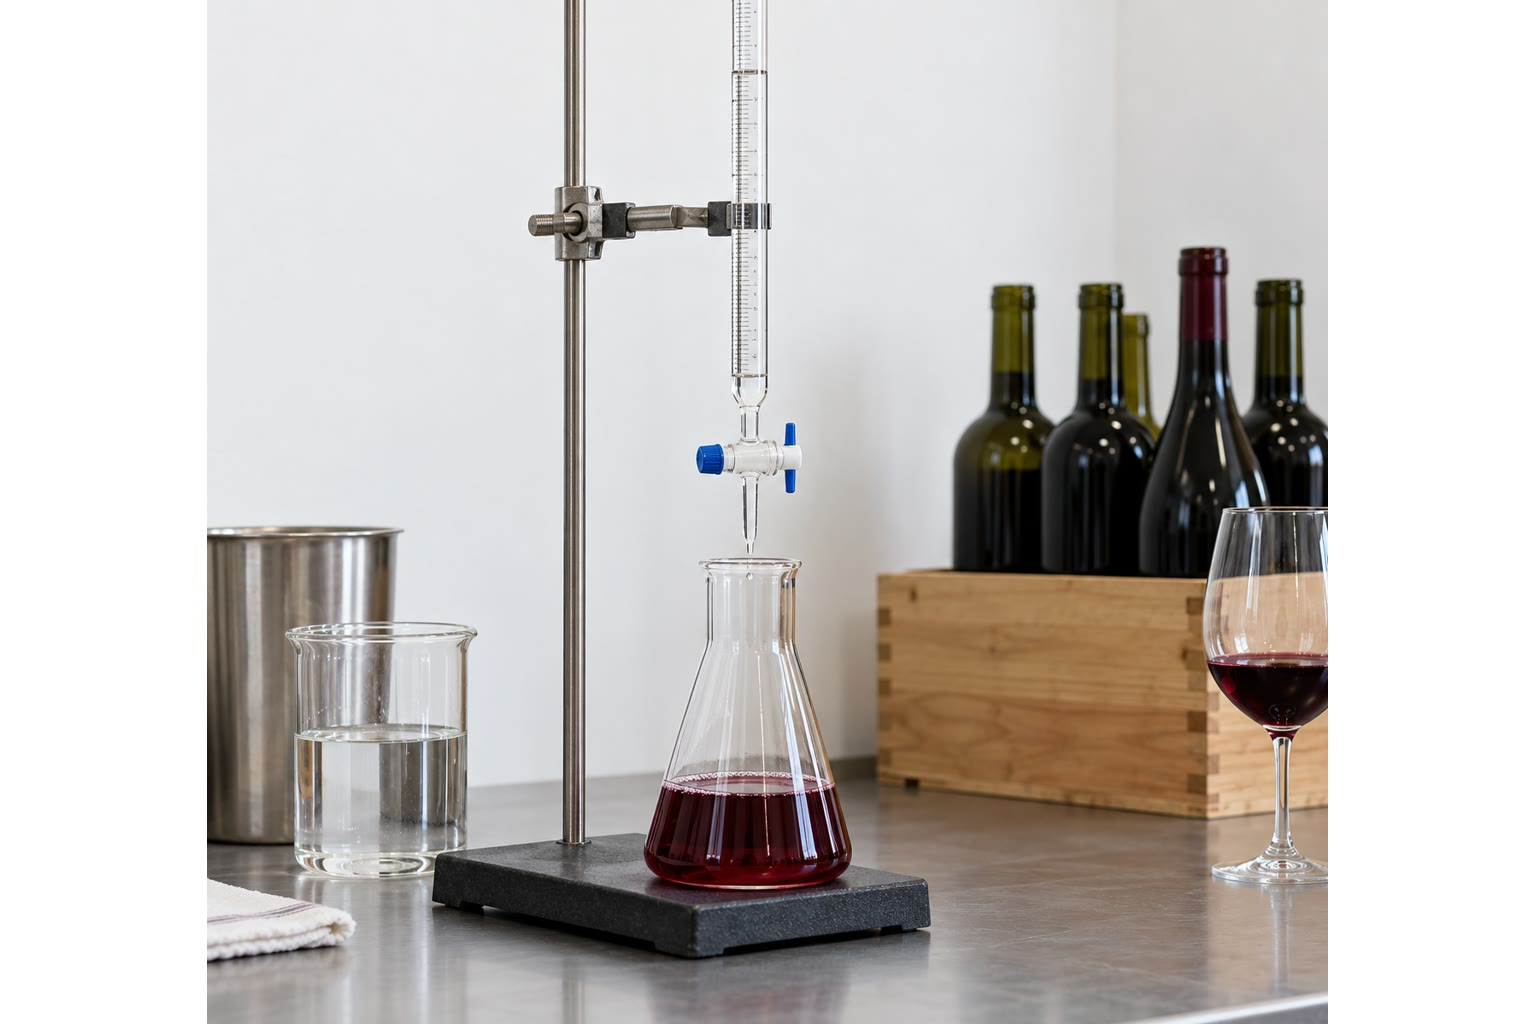
\includegraphics[width=0.45\linewidth]{images/book1/ai/g12-wine-lab.jpg}

{\small La mesa de \omterm{def:g11:titration:titration}{valoraciones} de un enólogo.}
\end{omfigure}

\section{La valoración pH-métrica}

\begin{definition}[Valoración pH-métrica, semiequivalencia]\label{def:g12:ph-conductivity-titrations:ph-metric}
En una \emph{valoración pH-métrica}\index{valoracion pH-metrica@valoración pH-métrica} se mide
el \omterm{def:g9:acids-bases-ph:ph}{pH} de la \omterm{def:g11:titration:titration}{disolución valorada} tras cada adición de \omterm{def:g11:titration:titration}{valorante}, y se
dibuja la curva del \omterm{def:g9:acids-bases-ph:ph}{pH} en función del volumen añadido. La
\emph{semiequivalencia}\index{semiequivalencia} es el punto en el que se
ha añadido la mitad del \omterm{def:g11:titration:equivalence}{volumen de equivalencia}.
\end{definition}

\begin{omfigure}
\begin{tikzpicture}[font=\small, scale=0.65]
  \pic[transform shape] at (0,0) {stand={6.3}{2.0}};
  \pic[transform shape] at (2.0,0.68) {stirrer};
  \pic[transform shape] at (2.0,0.68) {beaker={0.45}{omWater}};
  \pic[transform shape] at (2.0,2.9) {burette={0.8}{omWater}};
  \pic[transform shape] (pr) at (2.6,0.95) {probe};
  \pic[transform shape] (m) at (6.4,3.4) {meter={pH}};
  \draw[black!70, thick] (pr-top) .. controls +(0,1.0) and +(0,-1.2) .. (m-a);
  \draw[omProp, thick, <-] (2.35,7.2) -- (4.3,7.6) node[right, text=black] {bureta: NaOH};
  \draw[omProp, thick, <-] (1.4,1.1) -- (-1.4,1.6) node[left, text=black, align=right] {ácido que se valora};
  \draw[omProp, thick, <-] (2.75,2.4) -- (4.3,2.0) node[right, text=black] {sonda de pH};
\end{tikzpicture}

{\small Una \omterm{def:g12:ph-conductivity-titrations:ph-metric}{valoración pH-métrica}: la sonda está sumergida en la
disolución agitada, y el aparato indica el \omterm{def:g9:acids-bases-ph:ph}{pH} tras cada adición.}
\end{omfigure}

\begin{inthelab}[Calibrar un pHmetro]
Antes de usarla, la sonda se enjuaga con agua destilada y se sumerge en
dos \omterm{def:g12:buffers-predominance:buffer}{disoluciones tampón} de \omterm{def:g9:acids-bases-ph:ph}{pH} conocido, normalmente 7.0 y 4.0 (o 10.0):
el aparato se ajusta para que lea esos valores. Entre una disolución y
otra, la sonda se enjuaga y se seca con suaves toques, sin frotarla
nunca; se guarda con la punta húmeda.
\end{inthelab}

\begin{omfigure}
\begin{minipage}{0.49\linewidth}
\begin{tikzpicture}
\begin{axis}[width=\linewidth, height=6cm, xmin=0, xmax=30, ymin=0, ymax=14,
    xlabel={$V_{\text{NaOH}}$ (\si{mL})}, ylabel={pH}, axis lines*=left,
    ymajorgrids, grid style={gray!20}, tick label style={font=\scriptsize},
    label style={font=\small}, title={\small \ce{HCl} con \ce{NaOH}},
    title style={yshift=-4pt}]
  \addplot[very thick, omDef] table[x=V, y=pH] {figdata/out/grade-12-ph-conductivity-titrations-a.dat};
  \addplot[thick, omProp, densely dotted] table[x=V, y expr=\thisrow{dpH}/4]
    {figdata/out/grade-12-ph-conductivity-titrations-a.dat};
  \addplot[dashed, black!60] coordinates {(20,0) (20,7)};
  \node[font=\scriptsize, anchor=north west] at (axis cs:20.3,6.5) {$V_E = 20.0$};
\end{axis}
\end{tikzpicture}
\end{minipage}\hfill
\begin{minipage}{0.49\linewidth}
\begin{tikzpicture}
\begin{axis}[width=\linewidth, height=6cm, xmin=0, xmax=16, ymin=0, ymax=14,
    xlabel={$V_{\text{NaOH}}$ (\si{mL})}, ylabel={pH}, axis lines*=left,
    ymajorgrids, grid style={gray!20}, tick label style={font=\scriptsize},
    label style={font=\small}, title={\small \ce{CH3COOH} con \ce{NaOH}},
    title style={yshift=-4pt}]
  \addplot[very thick, omDef] table[x=V, y=pH] {figdata/out/grade-12-ph-conductivity-titrations-b.dat};
  \addplot[thick, omProp, densely dotted] table[x=V, y expr=\thisrow{dpH}/4]
    {figdata/out/grade-12-ph-conductivity-titrations-b.dat};
  \addplot[dashed, black!60] coordinates {(10.1,0) (10.1,8.7)};
  \addplot[dashed, black!60] coordinates {(0,4.76) (5.05,4.76) (5.05,0)};
  \node[font=\scriptsize, anchor=south west] at (axis cs:0.2,4.8) {$pK_a = 4.76$};
  \node[font=\scriptsize, anchor=north west] at (axis cs:10.4,3.0) {$V_E = 10.1$};
\end{axis}
\end{tikzpicture}
\end{minipage}

{\small Curvas de \omterm{def:g9:acids-bases-ph:ph}{pH} calculadas (en azul) y su derivada $d\mathrm{pH}/dV$
(en naranja, de puntos, dividida por 4). Izquierda: \qty{20.0}{mL} de
ácido clorhídrico a \qty{0.100}{mol/L}; \omterm{def:g11:titration:equivalence}{equivalencia} a \omterm{def:g9:acids-bases-ph:ph}{pH} 7.00. Derecha:
\qty{10.0}{mL} de vinagre diluido; en la \omterm{def:g12:ph-conductivity-titrations:ph-metric}{semiequivalencia} el \omterm{def:g9:acids-bases-ph:ph}{pH} es igual
al $pK_a$, y la \omterm{def:g11:titration:equivalence}{equivalencia} se da a un \omterm{def:g9:acids-bases-ph:ph}{pH} básico.}
\end{omfigure}


\begin{method}[El método de la derivada]\label{met:g12:ph-conductivity-titrations:derivative}
Calcula, entre medidas sucesivas, la pendiente
$\Delta\mathrm{pH}/\Delta V$, y represéntala en función de $V$ (lo hace
una hoja de cálculo o una calculadora). El \omterm{def:g11:titration:equivalence}{volumen de equivalencia} es
aquel en el que esta pendiente es máxima: el pico de la curva derivada.
\end{method}

\begin{method}[El método de las tangentes]\label{met:g12:ph-conductivity-titrations:tangent}
\begin{enumerate}
  \item Traza dos tangentes paralelas a la curva, una antes y otra
        después del salto, a ambos lados de él.
  \item Traza la paralela situada a medio camino entre ellas.
  \item El punto donde corta la curva es el punto de \omterm{def:g11:titration:equivalence}{equivalencia}: lee
        $V_E$ (y el \omterm{def:g9:acids-bases-ph:ph}{pH} en la \omterm{def:g11:titration:equivalence}{equivalencia}).
\end{enumerate}
\end{method}

\begin{proposition}[En la semiequivalencia, $\mathrm{pH} = pK_a$]\label{prop:g12:ph-conductivity-titrations:half}
En la \omterm{def:g11:titration:titration}{valoración} de un \omterm{def:g12:ka-and-pka:strong-acid}{ácido débil} \ce{HA} con una \omterm{def:g12:ka-and-pka:strong-acid}{base fuerte}, en la
\omterm{def:g12:ph-conductivity-titrations:ph-metric}{semiequivalencia} $\mathrm{pH} = pK_a$.
\end{proposition}

\begin{proof}
La reacción \ce{HA + OH- -> A- + H2O} es total. En la \omterm{def:g12:ph-conductivity-titrations:ph-metric}{semiequivalencia},
la mitad del ácido se ha transformado en \ce{A-}: $[\ce{A-}] = [\ce{HA}]$,
y la relación de Henderson da $\mathrm{pH} = pK_a + \log 1 = pK_a$.
\end{proof}

\begin{remark}[Elegir un indicador a partir de la curva]\label{rem:g12:ph-conductivity-titrations:indicator}
% ledger: ind:BBT, ind:phenolphthalein
El indicador debe cambiar de color dentro del salto. Para el ácido
clorhídrico, el salto va aproximadamente de \omterm{def:g9:acids-bases-ph:ph}{pH} 4 a 10 y sirven muchos
indicadores, el mejor el azul de bromotimol; para el ácido etanoico, el
salto es más corto y básico, alrededor de 7 a 11: sirve la fenolftaleína
(8.0--10.0), y el azul de bromotimol viraría demasiado pronto.
\end{remark}

\section{Conductividad y valoraciones conductimétricas}

\begin{definition}[Conductividad, conductividad molar iónica]\label{def:g12:ph-conductivity-titrations:conductivity}
La \emph{conductividad}\index{conductividad} $\sigma$ de una disolución
mide lo bien que conduce la electricidad; se lee en un conductímetro, en
\si{mS/cm} (o \si{S/m}). Cada \omterm{def:g9:ions:ion}{ion} $i$ contribuye a ella en proporción a
su concentración, con un coeficiente $\lambda_i$, su
\emph{conductividad molar iónica}\index{conductividad molar ionica@conductividad molar iónica}.
\end{definition}

\begin{proposition}[Ley de Kohlrausch]\label{prop:g12:ph-conductivity-titrations:kohlrausch}
% ledger: lam:H+, lam:OH-, lam:Na+, lam:Cl-
Para una disolución diluida, $\sigma = \sum_i \lambda_i [X_i]$. A
\qty{25}{\celsius}, en \si{S.cm^2/mol}: \ce{H3O+} 349.8, \ce{OH-} 198.3,
\ce{Cl-} 76.2, \ce{Na+} 50.3. Los \omterm{def:g12:ka-and-pka:oxonium}{iones oxonio} e hidróxido conducen mucho
mejor que todos los demás \omterm{def:g9:ions:ion}{iones}.
\end{proposition}

\begin{proof}
Se admite (volumen del primer año). Los valores de \ce{Cl-} y de
\ce{Na+} proceden de las \omterm{def:g12:ph-conductivity-titrations:conductivity}{conductividades} medidas de disoluciones de
ácido clorhídrico y de cloruro de sodio, a las que se resta la del
\ce{H3O+}.
\end{proof}

\begin{definition}[Valoración conductimétrica]\label{def:g12:ph-conductivity-titrations:conductimetric}
En una \emph{valoración conductimétrica}\index{valoracion conductimetrica@valoración conductimétrica}
se mide la \omterm{def:g12:ph-conductivity-titrations:conductivity}{conductividad} tras cada adición de \omterm{def:g11:titration:titration}{valorante}. La \omterm{def:g11:titration:titration}{disolución
valorada} se diluye en un gran volumen de agua, para que el volumen
añadido apenas la modifique: así los puntos quedan sobre rectas, que
cambian de pendiente en la \omterm{def:g11:titration:equivalence}{equivalencia}.
\end{definition}

\begin{omfigure}
\begin{minipage}{0.4\linewidth}\centering
\begin{tikzpicture}[font=\small, scale=0.75]
  \pic[transform shape] at (0,0) {beaker={0.6}{omWater}};
  \pic[transform shape] (cc) at (0.2,0.2) {condcell};
  \pic[transform shape] (m) at (2.6,3.4) {meter={mS/cm}};
  \draw[black!70, thick] (cc-top) .. controls +(0,0.8) and +(0,-1) .. (m-a);
  \node[anchor=north, align=center] at (0.6,-0.15) {célula de conductimetría\\ en la disolución};
\end{tikzpicture}
\end{minipage}\hfill
\begin{minipage}{0.56\linewidth}
\begin{tikzpicture}
\begin{axis}[width=\linewidth, height=5.4cm, xmin=0, xmax=20, ymin=0,
    ymax=4.6, xlabel={$V_{\text{NaOH}}$ (\si{mL})}, ylabel={$\sigma$ (\si{mS/cm})},
    axis lines*=left, ymajorgrids, grid style={gray!20},
    tick label style={font=\scriptsize}, label style={font=\small}]
  \addplot[only marks, mark=*, mark size=1.4pt, omDef] table[x=V, y=sigma]
    {figdata/out/grade-12-ph-conductivity-titrations-c.dat};
  \addplot[dashed, black!60] coordinates {(10,0) (10,4.6)};
  \node[font=\scriptsize, anchor=south west] at (axis cs:10.3,0.2) {$V_E = 10.0$};
\end{axis}
\end{tikzpicture}
\end{minipage}

{\small Izquierda: una célula de conductimetría. Derecha: \qty{100}{mL}
de ácido clorhídrico a \qty{0.0100}{mol/L} valorados con hidróxido de
sodio a \qty{0.100}{mol/L} (calculado con la ley de Kohlrausch). La
\omterm{def:g12:ph-conductivity-titrations:conductivity}{conductividad} baja y después sube: dos rectas que se cortan en la
\omterm{def:g11:titration:equivalence}{equivalencia}.}
\end{omfigure}

\begin{example}[Leer las dos rectas]\label{ex:g12:ph-conductivity-titrations:lines}
Antes de la \omterm{def:g11:titration:equivalence}{equivalencia}, cada \ce{OH-} añadido elimina un \ce{H3O+}
($\lambda = 349.8$) y aporta un \ce{Na+} ($\lambda = 50.3$): la
\omterm{def:g12:ph-conductivity-titrations:conductivity}{conductividad} baja bruscamente. Después de la \omterm{def:g11:titration:equivalence}{equivalencia}, el \ce{Na+}
y el \ce{OH-} ($\lambda = 198.3$) simplemente se acumulan: sube. Las dos
rectas se cortan en $V_E = \qty{10.0}{mL}$, así que el ácido estaba a
$0.100 \times 10.0 / 100 = \qty{0.0100}{mol/L}$.
\end{example}

\begin{method}[La equivalencia en una valoración conductimétrica]\label{met:g12:ph-conductivity-titrations:two-lines}
Traza la mejor recta por los puntos anteriores a la \omterm{def:g11:titration:equivalence}{equivalencia} y la
mejor recta por los posteriores; lee $V_E$ en su intersección. Los
puntos cercanos a la \omterm{def:g11:titration:equivalence}{equivalencia}, donde las rectas se curvan, se
descartan.
\end{method}

\begin{remark}[Qué método usar y cuándo]\label{rem:g12:ph-conductivity-titrations:which}
Un indicador coloreado es lo más rápido cuando existe uno adecuado. Una
\omterm{def:g12:ph-conductivity-titrations:ph-metric}{valoración pH-métrica} da además el $pK_a$ de un \omterm{def:g12:ka-and-pka:strong-acid}{ácido débil}, y funciona
con disoluciones coloreadas o turbias. Una \omterm{def:g12:ph-conductivity-titrations:conductimetric}{valoración conductimétrica} no
necesita ningún salto de \omterm{def:g9:acids-bases-ph:ph}{pH}: funciona con ácidos muy débiles o muy
diluidos, y con reacciones de \omterm{def:g9:ions:precipitate}{precipitación}, siempre que los \omterm{def:g9:ions:ion}{iones}
cambien.
\end{remark}

\begin{safety}{\ghs[0.82cm]{GHS05}\ghs[0.82cm]{GHS07}}
% ledger: ghs:NaOH
Las disoluciones de hidróxido de sodio queman la piel y los ojos, incluso
diluidas en el caso de los ojos: gafas en todo momento, y cualquier
salpicadura se enjuaga al instante con mucha agua.
\end{safety}

\section{Ejercicios}


\begin{exercise}[$\star$]\label{exo:g12:ph-conductivity-titrations:1}
Lee el \omterm{def:g11:titration:equivalence}{volumen de equivalencia} en la curva del ácido clorhídrico valorado
con hidróxido de sodio a \qty{0.100}{mol/L}, y deduce la concentración
de los \qty{20.0}{mL} de ácido.
\end{exercise}

\begin{exercise}[$\star$]\label{exo:g12:ph-conductivity-titrations:2}
Se valora un \omterm{def:g12:ka-and-pka:strong-acid}{ácido débil} con hidróxido de sodio; $V_E = \qty{12.0}{mL}$.
A \qty{6.0}{mL}, el \omterm{def:g9:acids-bases-ph:ph}{pH} es 3.75. Da el $pK_a$ del ácido. ¿Qué ácido de la
escala de $pK_a$ podría ser?
\end{exercise}

\begin{exercise}[$\star$]\label{exo:g12:ph-conductivity-titrations:3}
¿Qué indicador elegirías para la \omterm{def:g11:titration:titration}{valoración} del ácido etanoico con
hidróxido de sodio? ¿Por qué no el rojo de metilo?
\end{exercise}

\begin{exercise}[$\star$]\label{exo:g12:ph-conductivity-titrations:4}
¿Por qué hay que calibrar un \omterm{def:g9:acids-bases-ph:ph-paper}{pHmetro} antes de usarlo? ¿Con qué?
\end{exercise}

\begin{exercise}[$\star$]\label{exo:g12:ph-conductivity-titrations:5}
Con las \omterm{def:g12:ph-conductivity-titrations:conductivity}{conductividades molares iónicas}, ordena los \omterm{def:g9:ions:ion}{iones} \ce{H3O+},
\ce{OH-}, \ce{Na+}, \ce{Cl-} del mejor conductor al peor.
\end{exercise}

\begin{exercise}[$\star\star$]\label{exo:g12:ph-conductivity-titrations:6}
\qty{20.0}{mL} de una disolución de ácido etanoico necesitan
\qty{14.6}{mL} de hidróxido de sodio a \qty{0.050}{mol/L}. Calcula su
concentración.
\end{exercise}

\begin{exercise}[$\star\star$]\label{exo:g12:ph-conductivity-titrations:7}
Cerca de la \omterm{def:g11:titration:equivalence}{equivalencia}, las lecturas son: \qty{9.6}{mL}, \omterm{def:g9:acids-bases-ph:ph}{pH} 5.7;
\qty{9.8}{mL}, 6.1; \qty{10.0}{mL}, 7.0; \qty{10.2}{mL}, 10.5;
\qty{10.4}{mL}, 11.0. Calcula $\Delta\mathrm{pH}/\Delta V$ entre puntos
sucesivos y localiza $V_E$.
\end{exercise}

\begin{exercise}[$\star\star$]\label{exo:g12:ph-conductivity-titrations:8}
En la \omterm{def:g12:ph-conductivity-titrations:conductimetric}{valoración conductimétrica} del ácido clorhídrico, explica el signo
de la pendiente antes y después de la \omterm{def:g11:titration:equivalence}{equivalencia}, a partir de los \omterm{def:g9:ions:ion}{iones}
presentes.
\end{exercise}

\begin{exercise}[$\star\star$]\label{exo:g12:ph-conductivity-titrations:9}
Esboza la curva conductimétrica del ácido etanoico valorado con
hidróxido de sodio. ¿Por qué sube la \omterm{def:g12:ph-conductivity-titrations:conductivity}{conductividad} incluso antes de la
\omterm{def:g11:titration:equivalence}{equivalencia}?
\end{exercise}

\begin{exercise}[$\star\star$]\label{exo:g12:ph-conductivity-titrations:10}
En la curva calculada del vinagre diluido, lee el \omterm{def:g9:acids-bases-ph:ph}{pH} al principio, en la
\omterm{def:g12:ph-conductivity-titrations:ph-metric}{semiequivalencia} y en la \omterm{def:g11:titration:equivalence}{equivalencia}. ¿Por qué el \omterm{def:g9:acids-bases-ph:ph}{pH} inicial es mucho
más alto que el del ácido clorhídrico a la misma concentración?
\end{exercise}

\begin{exercise}[$\star\star$]\label{exo:g12:ph-conductivity-titrations:11}
¿Por qué se diluye la \omterm{def:g11:titration:titration}{disolución valorada} en un gran volumen de agua
antes de una \omterm{def:g12:ph-conductivity-titrations:conductimetric}{valoración conductimétrica}?
\end{exercise}

\begin{exercise}[$\star\star\star$]\label{exo:g12:ph-conductivity-titrations:12}
Una disolución contiene a la vez ácido clorhídrico y ácido etanoico. Se
valora con hidróxido de sodio midiendo el \omterm{def:g9:acids-bases-ph:ph}{pH}. Explica por qué la curva
presenta dos saltos, y qué mide cada \omterm{def:g11:titration:equivalence}{volumen de equivalencia}.
\end{exercise}

\begin{exercise}[$\star\star\star$]\label{exo:g12:ph-conductivity-titrations:13}
Calcula la \omterm{def:g12:ph-conductivity-titrations:conductivity}{conductividad} al principio de la \omterm{def:g12:ph-conductivity-titrations:conductimetric}{valoración conductimétrica}
del capítulo (ácido clorhídrico a \qty{0.0100}{mol/L}) y en la
\omterm{def:g11:titration:equivalence}{equivalencia} (\qty{110}{mL} de disolución de cloruro de sodio). Compara
con la figura.
\end{exercise}

\begin{exercise}[$\star\star\star$]\label{exo:g12:ph-conductivity-titrations:14}
Un \omterm{def:g9:acids-bases-ph:ph-paper}{pHmetro} mal calibrado marca todos los \omterm{def:g9:acids-bases-ph:ph}{pH} 0.2 por encima. ¿Qué error
provoca en el \omterm{def:g11:titration:equivalence}{volumen de equivalencia} de una \omterm{def:g12:ph-conductivity-titrations:ph-metric}{valoración pH-métrica}? ¿Y en
el $pK_a$ leído en la \omterm{def:g12:ph-conductivity-titrations:ph-metric}{semiequivalencia}?
\end{exercise}

\begin{exercise}[$\star\star\star$]\label{exo:g12:ph-conductivity-titrations:15}
¿Por qué una \omterm{def:g12:ph-conductivity-titrations:conductimetric}{valoración conductimétrica} puede seguir la reacción de los
\omterm{def:g9:ions:ion}{iones} plata con los \omterm{def:g9:ions:ion}{iones} cloruro, \ce{Ag+ + Cl- -> AgCl(s)}, y una
\omterm{def:g12:ph-conductivity-titrations:ph-metric}{valoración pH-métrica} no? Describe la curva esperada al añadir nitrato
de plata a cloruro de sodio (toma la $\lambda$ del \ce{NO3-} próxima a la
del \ce{Cl-}).
\end{exercise}

\section{Problema: ¿tiene el vinagre un 6\,\%?}

\begin{problem}[{Problema de fin de semana --- ¿contiene de verdad un vinagre con la
etiqueta ``6 \% de acidez'' seis gramos de ácido etanoico por cada cien gramos?}]
\label{pb:g12:ph-conductivity-titrations:1}
% ledger: pka:ethanoic, ind:phenolphthalein, lam:OH-, lam:Na+, aw:C, aw:H, aw:O
Se comprueba un vinagre con la etiqueta ``6 \% de acidez''. Se pesan
\qty{100.0}{mL}: \qty{101}{g}. El vinagre se diluye diez veces, y después
se valoran \qty{10.0}{mL} de la disolución diluida con hidróxido de
sodio a \qty{0.100}{mol/L}, con un \omterm{def:g9:acids-bases-ph:ph-paper}{pHmetro}; la curva calculada del
capítulo (a la derecha) coincide con las medidas.

\medskip
\noindent\textbf{Parte I --- Preparar la muestra.}
\begin{enumerate}
  \item ¿Qué significa ``6 \% de acidez''?
  \item Si la etiqueta es correcta, ¿qué masa de ácido etanoico contienen
        \qty{100.0}{mL} de vinagre? ¿A qué \omterm{def:g10:concentration-and-dilution:molar-concentration}{concentración molar}
        corresponde?
  \item ¿Por qué se diluye el vinagre antes de la \omterm{def:g11:titration:titration}{valoración}?
  \item ¿Qué material de vidrio se usa para diluirlo diez veces?
\end{enumerate}

\medskip
\noindent\textbf{Parte II --- La \omterm{def:g12:ph-conductivity-titrations:ph-metric}{valoración pH-métrica}.}
\begin{enumerate}[resume]
  \item Escribe la ecuación de la reacción de \omterm{def:g11:titration:titration}{valoración}.
  \item Lee el \omterm{def:g11:titration:equivalence}{volumen de equivalencia} en la curva.
  \item Calcula la concentración del vinagre diluido.
  \item Deduce la del vinagre.
  \item Lee el \omterm{def:g9:acids-bases-ph:ph}{pH} en la \omterm{def:g12:ph-conductivity-titrations:ph-metric}{semiequivalencia}. ¿Qué se obtiene de él?
  \item ¿Por qué el \omterm{def:g9:acids-bases-ph:ph}{pH} en la \omterm{def:g11:titration:equivalence}{equivalencia} es superior a 7?
  \item ¿Qué indicador habría dado el mismo resultado?
\end{enumerate}

\medskip
\noindent\textbf{Parte III --- Una comprobación conductimétrica.}
\begin{enumerate}[resume]
  \item Se repite la \omterm{def:g11:titration:titration}{valoración} con una célula de conductimetría,
        diluyendo la muestra en \qty{200}{mL} de agua. ¿Qué \omterm{def:g9:ions:ion}{iones}
        aparecen en la disolución antes de la \omterm{def:g11:titration:equivalence}{equivalencia}?
  \item ¿Por qué la \omterm{def:g12:ph-conductivity-titrations:conductivity}{conductividad} sube solo lentamente antes de la
        \omterm{def:g11:titration:equivalence}{equivalencia}?
  \item ¿Por qué sube más deprisa después?
  \item ¿Por qué la \omterm{def:g12:ph-conductivity-titrations:conductivity}{conductividad} es muy baja al principio?
  \item ¿Dónde deberían cortarse las dos rectas?
\end{enumerate}

\medskip
\noindent\textbf{Parte IV --- El veredicto.}
\begin{enumerate}[resume]
  \item Calcula la \omterm{def:g10:concentration-and-dilution:mass-concentration}{concentración en masa} de ácido etanoico en el vinagre.
  \item Calcula la masa de ácido etanoico en \qty{100.0}{mL} de vinagre.
  \item Deduce la masa de ácido etanoico por cada \qty{100}{g} de
        vinagre.
  \item Da la respuesta final: ¿cuál es la acidez del vinagre?
\end{enumerate}
\end{problem}
